% !Mode:: "TeX:UTF-8"

\section{学位论文的主要内容、实施方案、及可行性论证}

\subsection{主要研究内容}


本课题致力于解决中文语义依存图分析问题。首先,由于语义依存图分析的概念才提出不久,在该任务上目前无论是基于转移的分析方法还是基于图的分析方法的研究都十分有限,二者的优劣尚未有定论。因此需要同时对这两类方法进行探索,分别设计出分析语义依存图的算法。此外,由于目前中外文语义依存图分析任务的数据都相对较少,而我们使用的基于深度学习的方法对数据量的要求往往很大,因此需要探索利用其他技术提高系统性能的方法,包括结合语义依存图分析任务特点的模型融合技术以及多任务学习技术。

本课题针对上述难点和挑战,结合自然语言处理技术进行了相应的理论证明及实验尝试,其具体内容如下:

\begin{enumerate}
	\item \textbf{基于转移的分析方法}
	\ \ \ \ 目前基于转移的依存分析领域大部分工作的分析目标都是树结构,使用基于转移的方法分析依存图的难点在于如何在转移过程中找到一个词的多个父节点。
	针对这个问题,我们提出了新的转移系统,在找到一个词的父节点的同时不对其进行规约,直到其所有父节点都被找到再对其进行规约,从而实现了对语义依存图的分析。
	同时为了从转移状态中获取更丰富的信息作为预测转移动作的依据,我们在基于Stack LSTM的分类器的基础上提出了两个神经网络模块对转移系统中的缓存和子图进行建模,并将其应用在我们的BS-IT依存图分析系统中。该系统在中文语义依存图数据集上取得了目前最好结果。
	(本部分工作已完成,并分别在CCL 2016和AAAI 2018上发表了两篇文章)
	
	\item \textbf{基于图的分析方法}
	\ \ \ \ 由于依存树具有严格的结构限制(例如每个词只能拥有一个父节点),传统基于图的分析方法往往在计算出所有可能子结构的分数的基础上,使用\citeayu{eisner1996three}提出的Eisner算法(一种动态规划算法)进行解码,找出其中的最大生成树。
	然而依存图结构不具备这些结构限制,因此原来的解码算法在该任务上已经不适用。目前该方向的工作普遍采取了对每个子结构逐个判断的方法,并同时使用多种分解方式获得不同级别的子结构,然后用$AD^3$算法解码,解决子结构之间存在重叠的问题。由于没有了结构限制,仅靠第一步计算的分数作为判断依据产生的依存图精度会受到很大影响。
	因此我们首先将尝试将更适合的神经网络引入第一步计算子结构分数的过程中,提高其对子结构分数估计的准确性。同时我们还将尝试使用更高阶(即每个子结构包含更多弧)、更具有图结构特性的子结构分解方式,从而提高最终得到的语义依存图的精度。
	(本部分工作正在进行中)
	
	\item \textbf{基于不同长度LSTM的模型融合技术}
	\ \ \ \ 模型融合技术在依存分析领域内已经被一些工作证明是一种简单而有效的提升系统性能的方式,但目前普遍被使用的模型融合技术要么是用不同的系统预测出的多个结果进行投票获得最终结果,要么是在同一系统的训练中使用不同的随机初始化种子得到多个模型,然后在预测时同时使用这些模型。前者虽然有效且具有可解释性,但是要求设计多个不同且有效的分析系统,难度较大,往往被用于合并多个前人已经实现的系统。后者虽然只需要设计一个系统,但是可解释性不强。而且这两种方法都没有利用语义依存图的特性。
	因此我们将利用语义依存图短、中、长距离依赖关系的不同,尝试使用不同长度的LSTM对它们分别进行建模,然后对这些模型进行融合。该方法不仅利用了语义依存图的特性,而且具有较强可解释性,并可同时应用于基于转移的和基于图的方法中。
	(本部分工作正在进行中)
	
	\item \textbf{面向语义分析任务的多任务学习技术}
	\ \ \ \ 由于语义依存图分析任务刚提出不久,相关数据资源有限,目前已知的数据集在中文上只有SemEval-2016 Task 9中文语义依存图数据集,共有25430句人工标注的来自新闻和课文的中文句子。
	英文上只有SemEval-2015 Task 18广义语义依存图数据集,共有38916句人工标注的来自宾州树库华尔街日报部分的英文句子。
	%中文10068+15362 英文35657+1410+1849
	因此在中文语义依存图分析的研究中,更应该有效使用现有所有数据,同时利用句法依存分析、语义角色标注等其它领域数据帮助提高语义依存图分析器精度。
	我们将使用多任务学习技术,尝试把句中词的表示向量输入LSTM中,然后使用LSTM的隐层输出作为每个词的表示。然后将这些表示分别应用到语义依存图分析及相关的其它任务的模型中。这些模型在训练过程中会同时对共用的LSTM表示层进行更新,从而获得一个既具有语义信息,又具有句法等其它任务信息的表示层,最终实现同时提高语义依存图和其他相关任务分析器性能的目的。
	(本部分工作正在进行中)
	
\end{enumerate}

上述各研究内容的关系如图\ref{fig:relation}所示。
\begin{figure}[htbp]
	\centering
	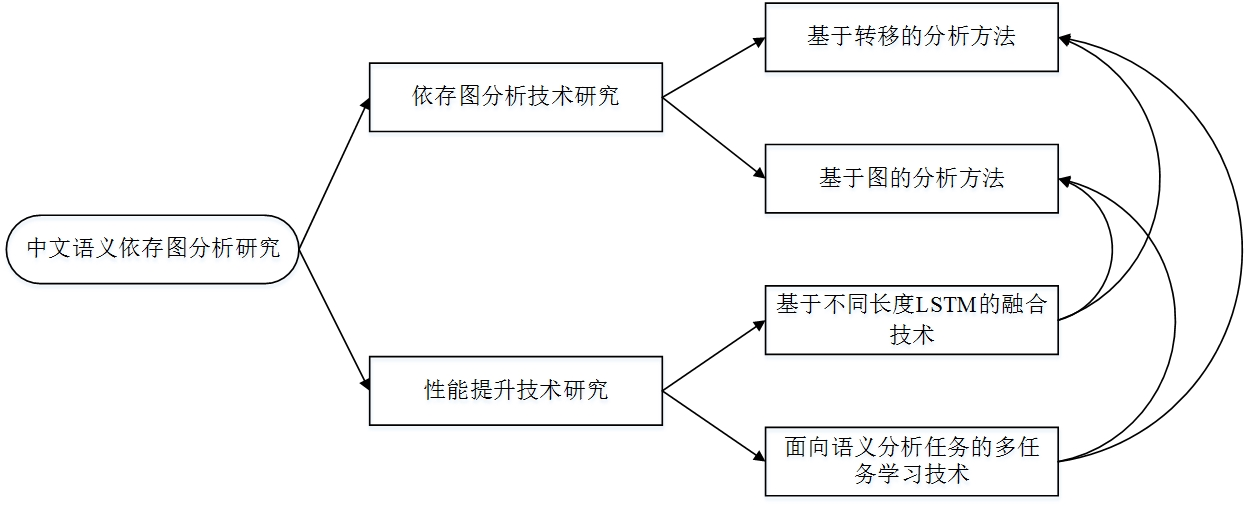
\includegraphics[width = 140mm]{picture/relation.jpg}
	\caption{研究内容概况图}
	\label{fig:relation}
\end{figure}



\subsection{实施方案}

由于四个研究点中的第一个已经完成,并且被录用,所以实施方案部分将主要介绍另外三个研究点。
研究工作将从如下几个方面展开:

\subsubsection{基于图的分析方法}

基于图的分析方法一般分为两步,第一步计算完全图中每个子结构的分数,第二步选出分数之和最大的子结构的组合作为预测出的目标结构。根据子结构的复杂度,基于图的分析模型可以分为一阶\citeyqy{mcdonald-crammer-pereira:2005:ACL}、二阶\citeyqy{mcdonald2006online}和高阶模型\citeyqy{koo-collins:2010:ACL},这里的阶数指的是每个子结构中依存弧的个数(例如一阶模型中每个子结构只包括一条弧)。高阶模型可以使用更复杂的子结构特征,因此其准确率更高,但解码算法的效率也会降低。

目前基于图的依存分析领域大部分工作的分析目标都是树结构的,由于依存树具有严格的结构限制(例如每个词只能有一个父节点),这些方法往往能够使用Eisner算法\citeyqy{eisner1996three}或在其基础上衍生出的其它动态规划算法\citeyqy{koo-collins:2010:ACL}进行解码。但是依存图结构中没有这些结构限制,因此上述方法在此不再适用。目前该方向的工作普遍采取了对每个子结构逐个判断的方法,这种方法虽然简单直观,但由于没有了结构限制,仅靠第一步计算的分数作为判断依据产生的依存图精度会受到很大影响。在此情况下要设计精度更高的基于图的依存分析方法,主要有两条路径,一是提高第一步中对每个子结构分数估计的准确性,二是选取更适合图结构的高阶模型,使得子结构本身就具有图的一定特性,从而提高最终得到的语义依存图的精度。接下来我们将分别介绍这两条路径的实施方案。

为了便于理解,我们首先以一阶模型为例,给出基于图的依存分析中第一步计算依存结构分数的形式化定义。在该模型中,一个依存结构的分数$s(\boldsymbol{x},\boldsymbol{y})$为其中所有子结构的分数之和(即所有弧的分数之和):

\begin{equation}
s(\boldsymbol{x},\boldsymbol{y})=\sum_{(i,j) \in \boldsymbol{y}} s(i,j)
\end{equation}

其中,$\boldsymbol{x}=x_1,\dots,x_n$表示输入句子,$\boldsymbol{y}$表示其对应的依存结构。我们可以将$\boldsymbol{y}$看作一个依存弧集合,因此$(i,j) \in \boldsymbol{y}$表示从词$x_i$指向词$x_j$的弧在$\boldsymbol{y}$中。

目前以依存图为分析目标的工作中,大多使用传统的基于离散特征的模型,使用高维稀疏的特征向量与特征权重向量的点积计算子结构的分值:

\begin{equation}
s(i,j) = \mathbf{w} \cdot \mathbf{f}(i,j)
\end{equation}

其中$\mathbf{f}(i,j)$表示从$x_i$指向$x_j$的弧对应的高维二元特征向量,$\mathbf{w}$表示特征权重向量。$\mathbf{f}(i,j)$中的每一维$f(i,j)$都用0和1表示一个特征是否出现,例如:

\begin{equation}
f(i,j)=
\begin{cases}
1& x_i = \text{"我" 且\ } x_j = \text{"是"} \\
0& \text{其他情况}
\end{cases}
\end{equation}

\citeayu{peng-thomson-smith:2017:Long}将依存句法分析领域中使用神经网络计算子结构分数的想法\citeyqy{kiperwasser2016simple}引入语义依存图分析中来,将句中词的词向量、词性向量作为双向LSTM的输入,然后将正向和反向LSTM的第$i$个时间节点的隐层状态拼接起来作为词$x_i$的表示向量$\mathbf{h}_i=[\overrightarrow{\mathbf{h}}_i;\overleftarrow{\mathbf{h}}_i]$。用这些低维致密的表示向量代替原有高维稀疏特征向量计算子结构分数,证明了该方法在依存图分析中的有效性。

\citeayu{peng-thomson-smith:2017:Long}的方法虽然成功将神经网络引入语义依存图分析任务中,但他们的对于词的表示比较单一,没有考虑一个词分别作为弧中的父节点和子节点时的不同情况。
目前基于图的句法分析方法中性能最好的是\citeayu{dozat2017deep}提出的基于深层双仿射(Biaffine)神经网络的分析器,他们凭借该分析器在CoNLL 2017多语言依存句法分析任务\citeyqy{zeman-EtAl:2017:K17-3}上取得了世界第一的成绩\citeyqy{dozat-qi-manning:2017:K17-3}。
该方法获得句中词的表示向量的步骤与\citeayu{peng-thomson-smith:2017:Long}相同,但在之后将这些表示输入4个不同的MLP分别获得每个词的4个表示向量:

\begin{equation}
\mathbf{h}^{(arc-dep)}_i = \text{MLP}^{(arc-dep)}(\mathbf{h}_i)
\end{equation}
\begin{equation}
\mathbf{h}^{(arc-head)}_i = \text{MLP}^{(arc-head)}(\mathbf{h}_i)
\end{equation}
\begin{equation}
\mathbf{h}^{(rel-dep)}_i = \text{MLP}^{(rel-dep)}(\mathbf{h}_i)
\end{equation}
\begin{equation}
\mathbf{h}^{(rel-head)}_i = \text{MLP}^{(rel-head)}(\mathbf{h}_i)
\end{equation}

其中$\mathbf{h}^{(arc-dep)}_i$和$\mathbf{h}^{(arc-head)}_i$分别表示$x_i$在计算弧的分数时作为子节点和作为父节点时的表示向量,$\mathbf{h}^{(rel-dep)}_i$和$\mathbf{h}^{(rel-head)}_i$分别表示$x_i$在计算弧标签分数时作为子节点和作为父节点时的表示向量。在此基础上利用双仿射分类器计算句中每个词作为词$x_i$的父节点时该弧的分数:

\begin{equation}
\begin{split}
\mathbf{s}^{(arc)}_i & = H^{(arc-head)}W^{(arc)}\mathbf{h}^{(arc-dep)}_i \\
& + H^{(arc-head)}\mathbf{b}^{\top(arc)}
\end{split}
\end{equation}

其中$\mathbf{s}^{(arc)}_i$是每个词作为$x_i$的父节点的分数向量,它的第$j$维表示弧$(j\rightarrow i)$的分数。$H^{(arc-head)} \in \mathbb{R}^{n \times d}$是句中$n$个词的$(arc-head)$表示向量拼接起来的矩阵。$W^{(arc)} \in \mathbb{R}^{d \times d}$是弧的权重矩阵,$\mathbf{h}^{(arc-dep)}_i$是词$x_i$的$(arc-dep)$表示向量,$\mathbf{b}^{(arc)}$是弧的偏移向量。使用这种方法,我们能够计算出任意两个词之间的弧的分数,在此基础上使用解码算法就能得到预测出的依存图结构。之后需要为每条弧计算出对应的弧标签,假设$y'_i$是我们预测出的词$x_i$的父节点,这条弧上弧标签的分数向量为:

\begin{equation}
\begin{split}
\mathbf{s}^{(rel)}_i & = \mathbf{h}_{y'^{(arc)}}^{\top(rel-head)}\mathbf{U}^{(rel)}\mathbf{h}^{(rel-dep)}_i \\
& + W^{(rel)}(\mathbf{h}^{(rel-dep)}_i \oplus \mathbf{h}^{(rel-head)}_{y'^{(arc)}_i}) \\
& + \mathbf{b}^{(rel)}
\end{split}
\end{equation}

其中$\mathbf{s}^{(rel)}_i \in \mathbb{R}^{k}$是$k$个弧标签的分数向量,每一维表示一个标签的分数。$\mathbf{h}_{y'^{(arc)}}^{(rel-head)}$是词$y'_i$的$(rel-head)$表示向量,$\mathbf{h}^{(rel-dep)}_i$是词$x_i$的$(rel-dep)$表示向量,$\mathbf{U}^{(rel)} \in \mathbb{R}^{d\times k \times d}$是弧标签的权重张量,$W^{(rel)} \in \mathbb{R}^{k \times 2d}$是弧标签的权重矩阵,$\mathbf{b}^{(rel)}$是弧标签的偏移向量。最终选择分数最高的弧标签作为这条弧上的标签$y'^{(rel)}_i$:

\begin{equation}
y'^{(rel)}_i = \arg \max_j s^{(rel)}_{ij}
\end{equation}

该方法不仅有效利用了神经网络强大的信息抽取能力,而且考虑了每个词作为弧中的父节点和子节点时的不同情况,因此在句法依存树分析任务中获得了目前最好结果。为了进一步提高基于图的语义依存图分析方法中第一步对每个子结构分数估计的准确性,我们会将该模型应用到依存图分析任务中来,为第二步的解码提供良好的基础。

\begin{figure}[hbtp]
	\centering
	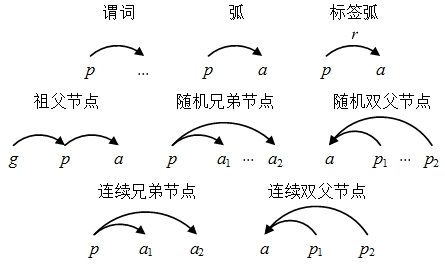
\includegraphics[width=100mm]{picture/parts.jpg}
	\caption{\citeayu{martins2014priberam}使用的子结构}
	\label{fig:parts}
\end{figure}

为了提高语义依存图分析的精度,我们还会尝试选取更适合图结构的高阶模型,使子结构具有图的一定特性。目前已有的基于图的语义依存图分析研究工作中,一般使用的是一阶或二阶模型。\citeayu{martins2014priberam}在其工作中首次使用了具有图特性的子结构,他们所使用的的所有子结构如图~\ref{fig:parts}所示。其中第一行三个为一阶分解,第二和第三行为二阶分解,随机双父节点和连续双父节点两种子结构为图结构所特有的。在依存句法分析领域,很多工作使用了超过二阶的模型,例如\citeayu{koo-collins:2010:ACL}和\citeayu{martins-almeida-smith:2013:Short}都使用了每个子结构包含三条弧的三阶模型。因此,我们将尝试将上述的随机双父节点和连续双父节点两种子结构扩展到三阶,即随机三父节点和连续三父节点,从而增强子结构的图特性,提高分析系统的精度。

\subsubsection{基于不同长度LSTM的模型融合技术}

模型融合技术目前已经在依存分析领域内取得了一些成功,被视为是一种简单而有效的提升系统性能的方式。但目前普遍被使用的模型融合技术要么是用不同的系统预测出的多个结果进行投票决定最终结果\citeyqy{du-EtAl:2015:SemEval},要么是在同一系统的训练中使用不同的随机初始化种子得到多个模型,然后在预测时同时使用这些模型\citeyqy{kuncoro-EtAl:2016:EMNLP2016,che-EtAl:2017:K17-3}。前者虽然有效且具有可解释性,但是要求设计多个不同且有效的分析系统,难度较大,往往被用于合并多个前人已经实现的系统。后者虽然只需要设计一个系统,但是可解释性不强。而且这两种方法都没有利用语义依存图的特性。

在语义依存图中,一个重要的区分依存弧的指标就是弧中两个词的距离。基于这一点观察,我们希望按照依存距离的不同建立多个模型,用它们分别对短、中、长距离的依存关系进行建模,然后对这些模型进行融合。因此,我们需要一个能够对可变长度序列进行编码的模型。

\begin{figure}[hbtp]
	\centering
	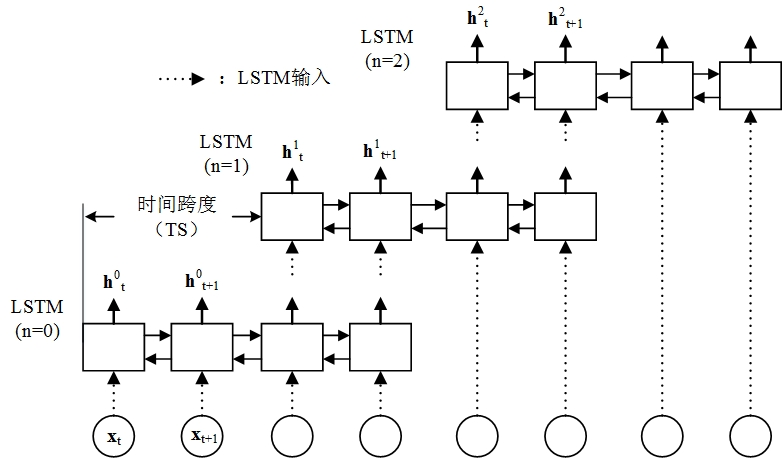
\includegraphics[width=130mm]{picture/ts-lstm.jpg}
	\caption{TS-LSTM网络结构示意图(LSTM个数$N=3$,窗口长度$W=4$,时间跨度$TS=2$)}
	\label{fig:ts-lstm}
\end{figure}

我们从\citeayu{lee2017ensemble}的动作识别的研究工作中得到了启发。他们提出了一种时间滑动长短时记忆网络(Temporal Sliding LSTM, TS-LSTM),由多个在输入序列上以一定的时间跨度滑动的LSTM组成。通过改变时间跨度$TS$和LSTM的窗口长度$W$可以实现提取不同长度依存信息的目的。该TS-LSTM的网络结构如图~\ref{fig:ts-lstm}所示。其中$x_t$表示句中第$t$个词的向量表示,

%该方法不但利用了语义依存图的结构特性,而且具有较强的可解释性,并且可以同时应用于基于转移的和基于图的分析方法中。

\subsubsection{面向语义分析任务的多任务学习技术}


\subsection{可行性分析}
\begin{enumerate}
	\item 本人长期关注自然语言处理相关技术、理论等。具有一定的理论基础,已经阅读并整理了大量的相关文献,对国内外研究现状有了较清晰的了解,详细掌握了目前中文语义依存图分析中存在的问题以及主要的研究方向。
	
	\item 我们的初期工作已经发表在CCL 2016,AAAI 2018等国内外重要学术会议上,其创新性得到了同行的认可。
	
	\item 所在的社会计算与信息检索研究中心经过多年的技术积累,已经基本掌握了自然语言处理中分词、词性标注、句法依存分析、语义角色标注等多种底层的关键技术。在上述各个方面都积累了大量的代码与数据,研究中心的语言技术平台享誉国内,加之本人对语义依存图分析技术已有较深刻的理解,这些技术和数据都为完成本课题提供了良好的支持。同时目前我实验室正在与北京语言大学合作完善中文语义依存图标注体系,标注更多中文语义依存图数据,这为本论文研究工作的开展起到了很大的帮助。
	
	
\end{enumerate}
\section{论文的进度安排与预期目标}

\subsection{进度安排}

2016年9月 - 2017年3月:博士论文选题,参考文献收集。

2017年4月 - 2017年10月:完成基于转移的语义依存图分析方法研究,完成论文写作并发表

2017年11月 - 2018年6月:完成针对语义依存图特点的模型融合技术的研究

2018年7月 - 2019年4月:完成基于图的语义依存图分析方法研究

2019年5月 - 2019年12月:完成利用多语言、多领域数据帮助中文语义依存图分析的研究

2020年1月 - 2020年6月:撰写毕业论文,申请毕业答辩。


\subsection{预期目标}

本课题致力于解决中文语义依存图分析中的关键问题,其中包括两部分,首先是语义依存图分析方法本身,然后是如何提高这些方法的性能。在前期的探索中,我们利用基于转移的依存分析方法,提出了新的能够分析语义依存图的转移系统,同时设计了新的网络结构,利用LSTM获取转移状态的信息用于转移动作的预测。这部分工作已经在中文语义依存图问题上取得了目前最好的结果,下一步的工作,我们要沿着依存分析的另一条道路,探索基于图的语义依存图分析方法。同时还要在这两类方法的基础上研究针对语义依存图特点的模型融合技术以及如何利用多语言、多领域数据帮助语义依存图分析。综合这些工作,我们预期目标为分别利用基于转移和基于图的方法解决中文语义依存图分析问题,利用多项技术提高这些方法的性能,并比较两类方法在该问题上的优劣,最终构建一个高效且能够利用更丰富的资源的实用的中文语义依存图分析系统。

\section{学位论文预期创新点}
与前人已发表的研究成果相比,本学位论文的预期创新点主要有以下几点:

(1)提出了一个利用注意力机制来直接生成顺滑块的方法。传统的序列标注等方法很难充分的利用全局信息,而我们的基于注意力机制的方法首先会对整个句子进行编码,之后再次序的生成顺滑块,其可以理解为一个全局的决策过程,因此能够充分的利用全局信息。

(2)提出了一个基于转移的顺滑方案。顺滑任务的一个主要的特点是非顺滑块和对应的顺滑块之间有很强的相似性,我们设计的基于转移的方案可以很好的利用这些块之间联系,实验结果表明基于转移的方案取得了目前最好的试验效果。

(3)正在实现的基于easy-first的顺滑方案。以前的方案大都是从左往右进行决策,这种方案的主要问题是决策是局部的,而且只能看到很少的右边的信息。我们设计的基于easy-first的方案的生成过程是一个由易到难的过程,避开了从左往右进行决策的问题,而且我们的方案在决策的过程中还能充分的利用块信息。

(4)正在实现的基于dual learning的顺滑方案。以前的方案大部分只关注模型本身的改进,很少有利用大量未标注数据的方案。我们的方案通过正向和逆向两个模型的互相交互,将大量的口语数据和标准的新闻数据引入进来,从而期望能利用更少的语料,取得不错的实验效果。


\section{为完成课题已具备和所需的条件、外协计划及经费}
\begin{enumerate}
	\item 相关工作的理论基础的积累:包括文献整理、平台搭建等工作(已完成);
	\item 基于注意力机制的顺滑方案:首次从生成的角度来解决顺滑问题(已完成);
	\item 基于转移的顺滑方案:该方案可以充分的利用不同块之间的信息(已完成);
	\item 基于easy-first的方案:已完成初步的方案设计和代码编写,进一步的实验结果即将得出;
	\item 基于dual learning的方案:已完成初步的方案设计,即将开始编写代码;
	\item 本论文的课题研究经费充足,能够保证相关工作正常进行。
	\item 本论文的课题研究得到了科大讯飞公司合肥研究院(总部)的鼎力支持。
\end{enumerate}


\section{预计研究过程中可能遇到的困难、问题,以及解决的途径}

\begin{enumerate}
	\item 在dual learning方案中如何约束逆向的生成过程:对于dual learning方案,逆向的生成过程是由顺滑的(不含不流畅块)句子生成含有不流畅块的句子,在理论上,在顺滑句子的基础上添加任何成分都是合理的,但是这样无限制的生成方案可能会带来严重的问题,也就是说正向和逆向不是严格对称的,因此如何消除或者减少这种不对称将是实验过程中需要重点关注的部分。
	\item 训练语料不足问题:由于复杂的神经网络需要大规模的训练语料,现有的English SwitchBoard数据只有八万句左右,当模型变复杂的时候,其规模略小。由于实验室跟讯飞有相关的合作,讯飞方面将负责标注大量的中文语料,从而能很好的验证我们模型在大规模语料上的效果。
	\item 实验结果不理想的问题:实验效果不理想可能是由多种不同的原因造成的。如果遇到这种问题,首先会排查代码是否有bug。其次,会对实验结果进行详细的分析,进而根据实验结果,决定是否对模型进行调整和优化。
\end{enumerate}

\section{发表论文情况}
\begin{enumerate}
	\item \textbf{Yuxuan Wang}, Wanxiang Che, Jiang Guo and Ting Liu. A Neural Transition-Based Approach for Semantic Dependency Graph Parsing. In Proceedings of the 32nd AAAI Conference on Artificial Intelligence (AAAI 2018). 2018.02. New Orleans, LA, USA.(已录用, CCF排名A类,重要国际会议,oral)
	\item \textbf{Yuxuan Wang}, Jiang Guo,  Wanxiang Che, and Ting Liu. Transition-Based Chinese Semantic Dependency Graph Parsing. In Proceedings of China National Conference on Chinese Computational Linguistics (CCL 2016,最佳论文奖,oral). 2016.10. Yantai, China.
\end{enumerate}

\clearpage

\newpage